Our workflow takes two inputs: a quantum circuit implementing a target unitary, $V$, and target output error $\epsilon^2$. This error could be with respect to the estimation of an observable or some distance metric on the output state of the circuit.  

The workflow builds on two principal strategies: (i) partitioning of the target circuit into smaller subcircuits, and (ii) averaging over ensembles of circuits to define an effective quantum channel. 
Partitioning decomposes the target circuit into a directed graph of
subcircuit blocks, each of which can be synthesized
independently. Ensemble averaging defines a quantum channel that
permits each subcircuit to be compiled only to accuracy $\epsilon$,
while rigorously ensuring that the overall circuit output error
remains bounded by $O(\epsilon^2)$. By combining circuit partitioning
with relaxed per-block synthesis accuracy, this approach substantially
improves compilation efficiency. Furthermore, it enables systematic
trade-offs in resource optimization, such as reducing the count of
two-qubit gates in NISQ implementations or minimizing the number of
non-Clifford gates in FT realizations. We view our workflow as the last step in a full compilation pipeline. Since we are generating approximate solutions, we can find further gate reductions on top of \emph{already optimized} circuits. 

\begin{figure}[t]
\begin{center}
    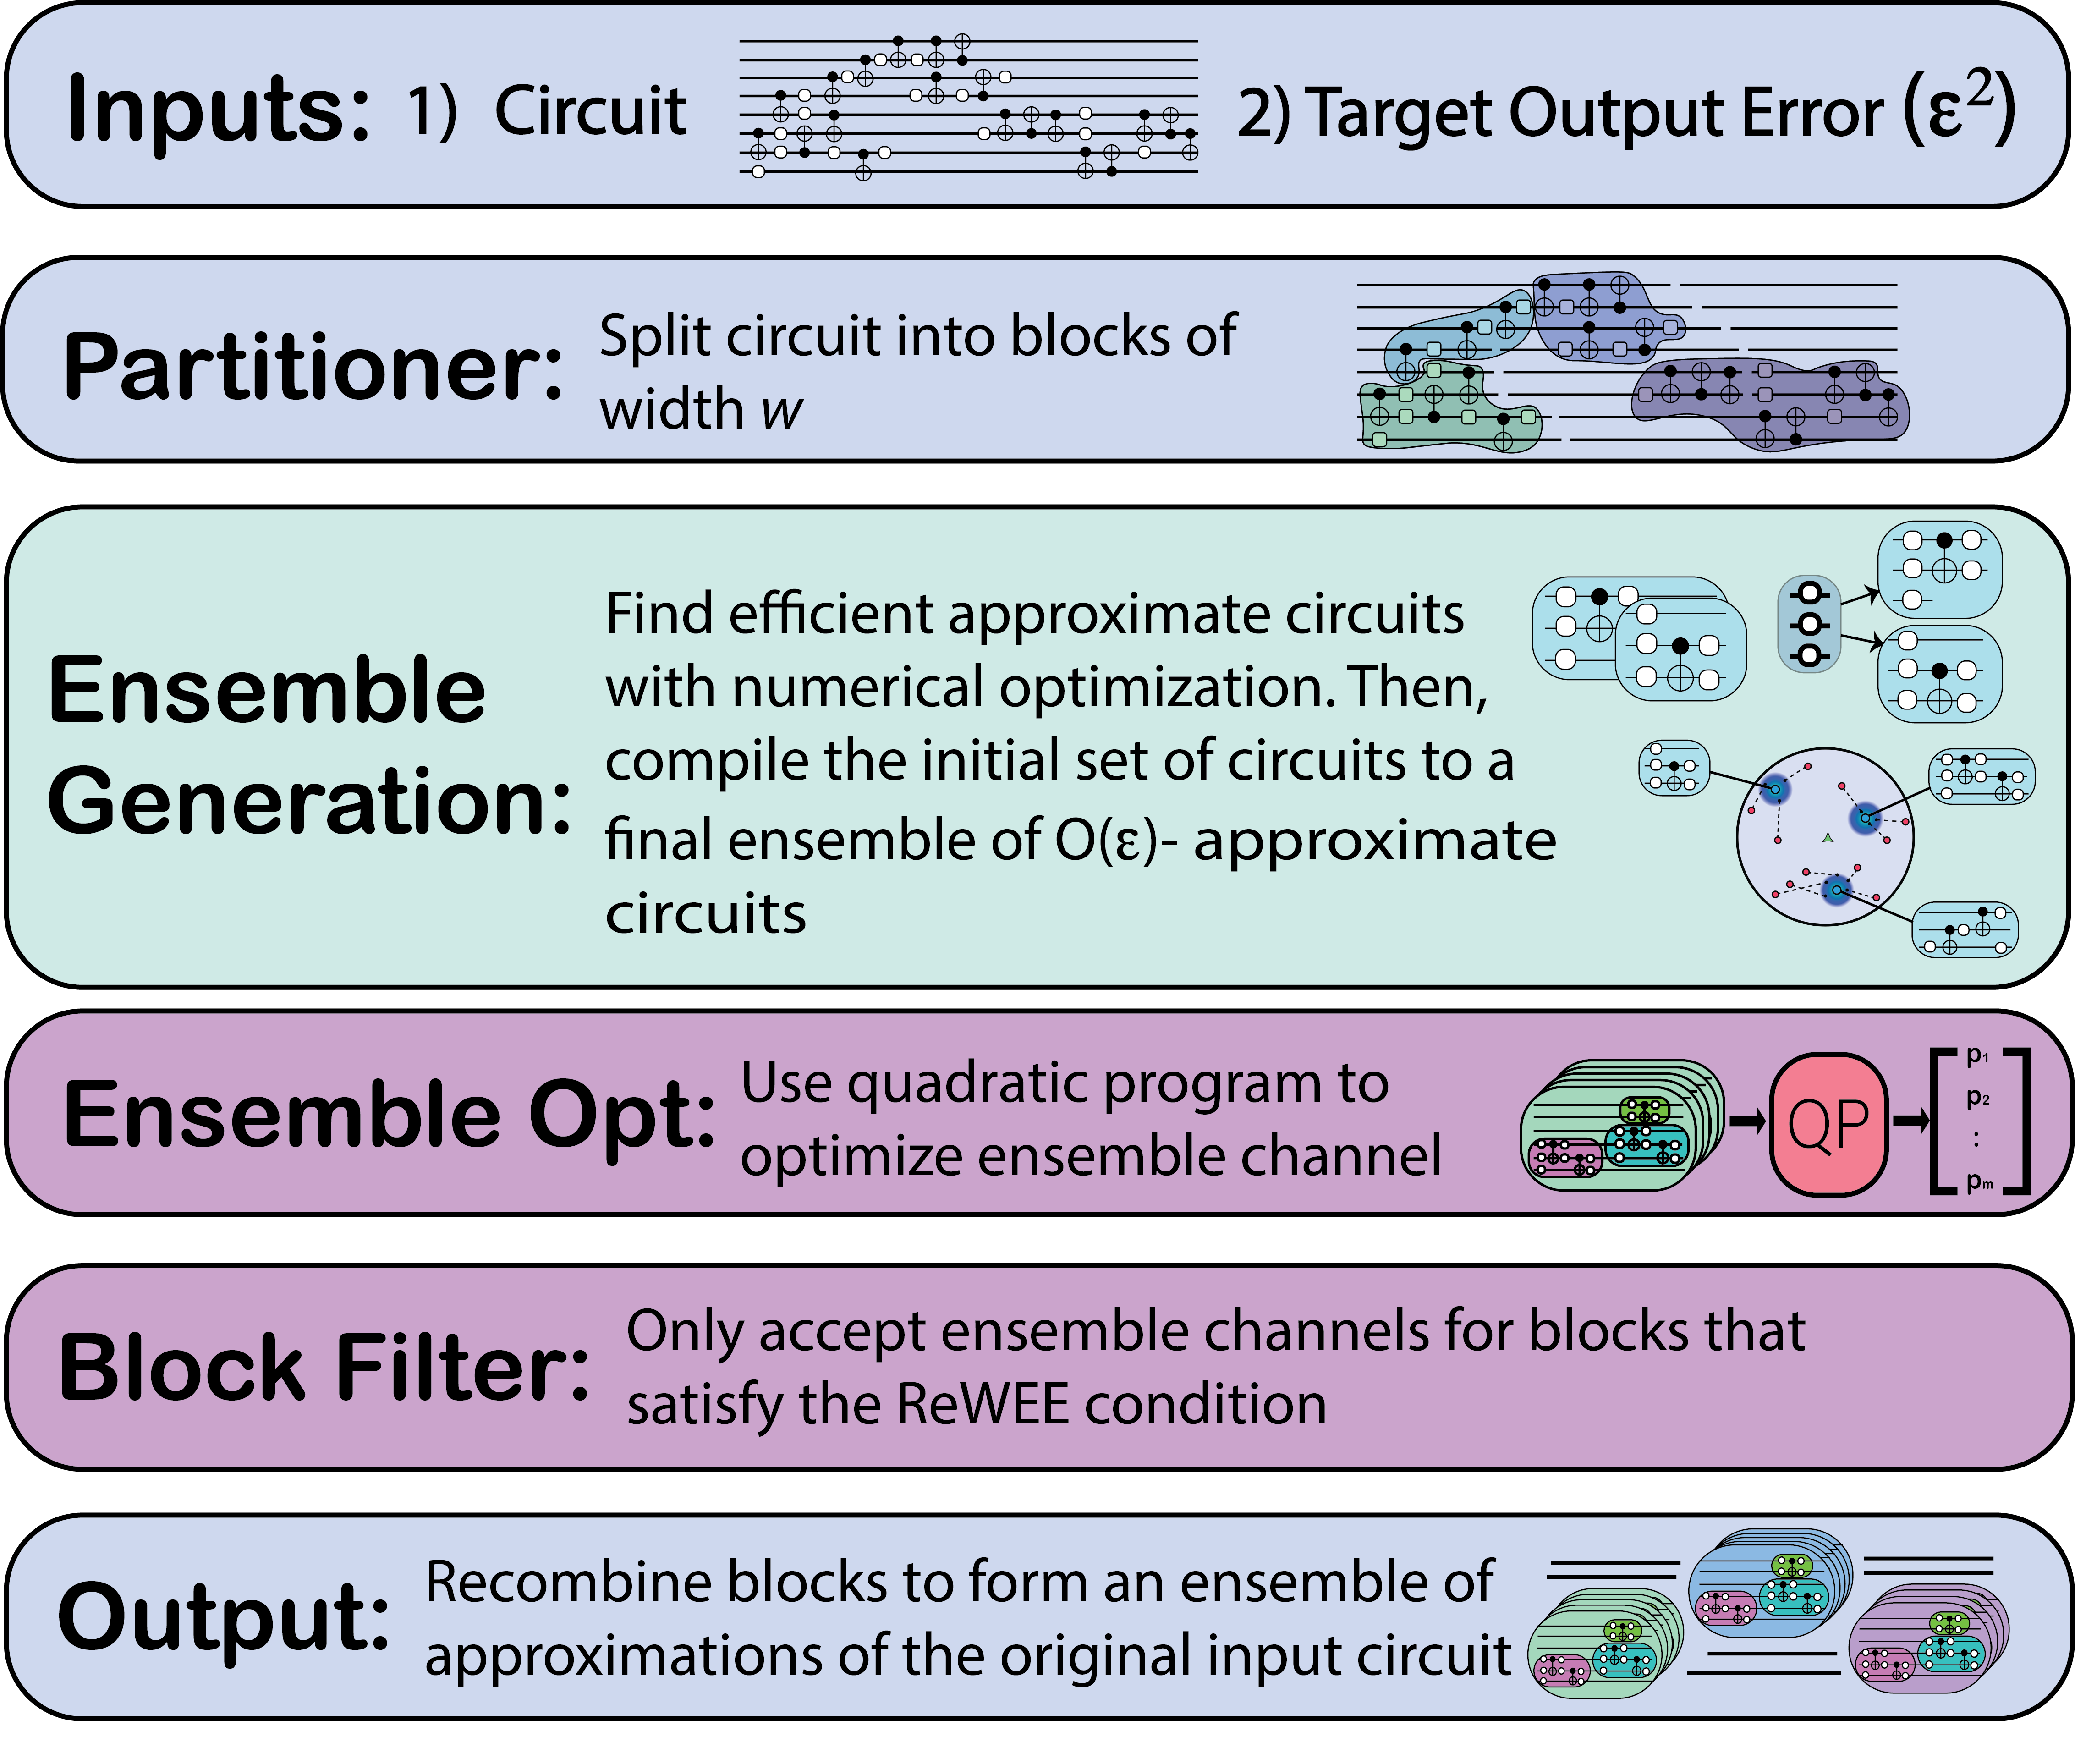
\includegraphics[width=\linewidth]{figures/FullWorkflow_results_new.png}
\captionof{figure}{High level overview of our workflow. Each step is summarized in the text and discussed in detail in the Methods.}
\label{fig:resut_workflow}
\end{center}
\end{figure}

A high-level overview of the compilation workflow is presented in
Figure~\ref{fig:resut_workflow}, with detailed descriptions of each
step provided in the Methods section. We briefly describe each step here and the theoretical foundations that motivate it. 

The \emph{Partitioner} splits the input circuit into $K$ non-overlapping subcircuits, or \emph{blocks}. Then the \emph{Ensemble Generation} step creates an ensemble of circuits that are $\epsilon$-approximations to the target unitary for each block; \ie $||U^\k_i - V^\k||_F \leq \epsilon$, for $1\leq i \leq M^\k_{\rm synth}$, where $U^\k_i$ is the $i$th member of the ensemble for partition $k$, $V^\k$ is the target unitary for partition $k$, and $||A||_F \equiv \sqrt{\tr(A\dg A)}$ is the Frobenius norm. This norm is chosen at this step for its computational efficiency. Resource-aware
synthesis may be applied at this stage, \eg penalizing costly gates
such as arbitrary angle rotations. Additionally, this step aims increase the diversity of the ensemble for each block while maintaining the approximation error of each member of the ensemble below $\epsilon$. Next, the \emph{Ensemble Optimization} step solves a convex quadratic program to determine an optimal \emph{weighted} ensemble for each block; \ie weights $0 \leq p^\k_i \leq 1$ (with $\sum_{i=1}^{M^\k} p^\k_i = 1$) are computed that minimize the \emph{weighted ensemble error}: $\normf{\sum_{i=1}^{M^\k} p^\k_i U^\k_i - V^\k}$. 

At the end of these steps, the critical property that we require is that the weighted ensemble error is quadratically reduced with respect to the original compilation tolerance $\epsilon$, \ie $\normf{\sum_{i=1}^{M^\k}p^\k_i U^\k_i - V^\k} \leq O(\epsilon^2)$. We refer to this as the \emph{reduced weighted ensemble error} (ReWEE) condition, and intuitively, it results from a synthesis algorithm that can generate a diversity of circuits whose convex hull contains a matrix that is closer to the target $V^{(k)}$ than any of the original circuits, as illustrated in Fig. \ref{fig:reduced_bias_combined}. A \emph{sufficient} condition for achieving ReWEE is an easily verifiable bias condition on the output of the \emph{Ensemble Generation} step: $\normf{\E{U_i^\k}-V^\k} \leq O(\epsilon^2)$, see Lemma 2 in Methods. The expectation above is taken with respect to the circuit distribution output by the Generation step.

Under the ReWEE condition, we show in the Methods that an immediate consequence of the \emph{Mixing Lemma} \cite{PhysRevA.95.042306,hastings2016turning}, is that the channel induced by averaging over the ensemble of circuits, $\mathcal{U}^\k[\rho] = \sum_{i=1}^{M^\k} p^\k_i U^\k_i \rho U_i^{(k)\dagger}$, has quadratically reduced error to the target channel, 
\begin{align}
    d_{\diamond}\left(\mathcal{U}^\k, \mathcal{V}^\k\right) \leq O(\epsilon^2),
    \label{eq:diamond_bound}
\end{align} 
where $\mathcal{V}^\k[\rho] = V^\k \rho V^{(k)\dagger}$ is the action of the target unitary, and $d_\diamond(\cdot,\cdot)$ is the diamond distance (defined in Methods), which has the interpretation as the worst-case discrepancy between the outputs of two channels \cite{watrous_2018}. 

The channel $\mathcal{U}^\k$ defines a discrete distribution over $M^\k$ circuits (set by $\{p^\k_i\}_{i=1}^{M^{(k)}}$ and denoted $\mathbb{P}_k$), and Eq. \eqref{eq:diamond_bound} says that averaging over circuits sampled from this distribution results in worst-case output error $O(\epsilon^2)$, compared to $\epsilon$ if any one of the members of ensemble is executed. This quadratic reduction in worst-case error is the key benefit to using the ensemble of compilations. 

Given optimized ensembles for all $K$ partitions, this defines a joint distribution $\mathbb{P} \equiv \mathbb{P}_1 \times ... \times \mathbb{P}_K$, from which circuits are sampled when executing the full-scale circuit. By the triangle inequality, the overall circuit error is bounded as $d_\diamond(\mathcal{U}^{(K)}\circ ... \circ \mathcal{U}^{(1)}, \mathcal{V}^{(K)}\circ ... \circ \mathcal{V}^{(1)}) \leq O(K \epsilon^2)$. The impact of the quadratic reduction in output error can be interpreted in two ways: (i) enabling coarser approximations at the subcircuit synthesis stage, or (ii) enabling application of the workflow to a larger number of partitions and thus larger circuits.

Note that if the \emph{Ensemble Generation} and \emph{Ensemble Optimization} steps are unable to find circuit ensembles that satisfy the ReWEE condition for some block, then the \emph{Block Filter} step replaces the ensemble channel for that block with the original circuit without approximations and sacrifices resource optimization in that block. Such filtering can occur if some blocks afford no resource optimization without incurring significant approximation error. Note that the output error bound is still guaranteed because the original circuit has zero approximation error.

\begin{figure}[t]
\centering
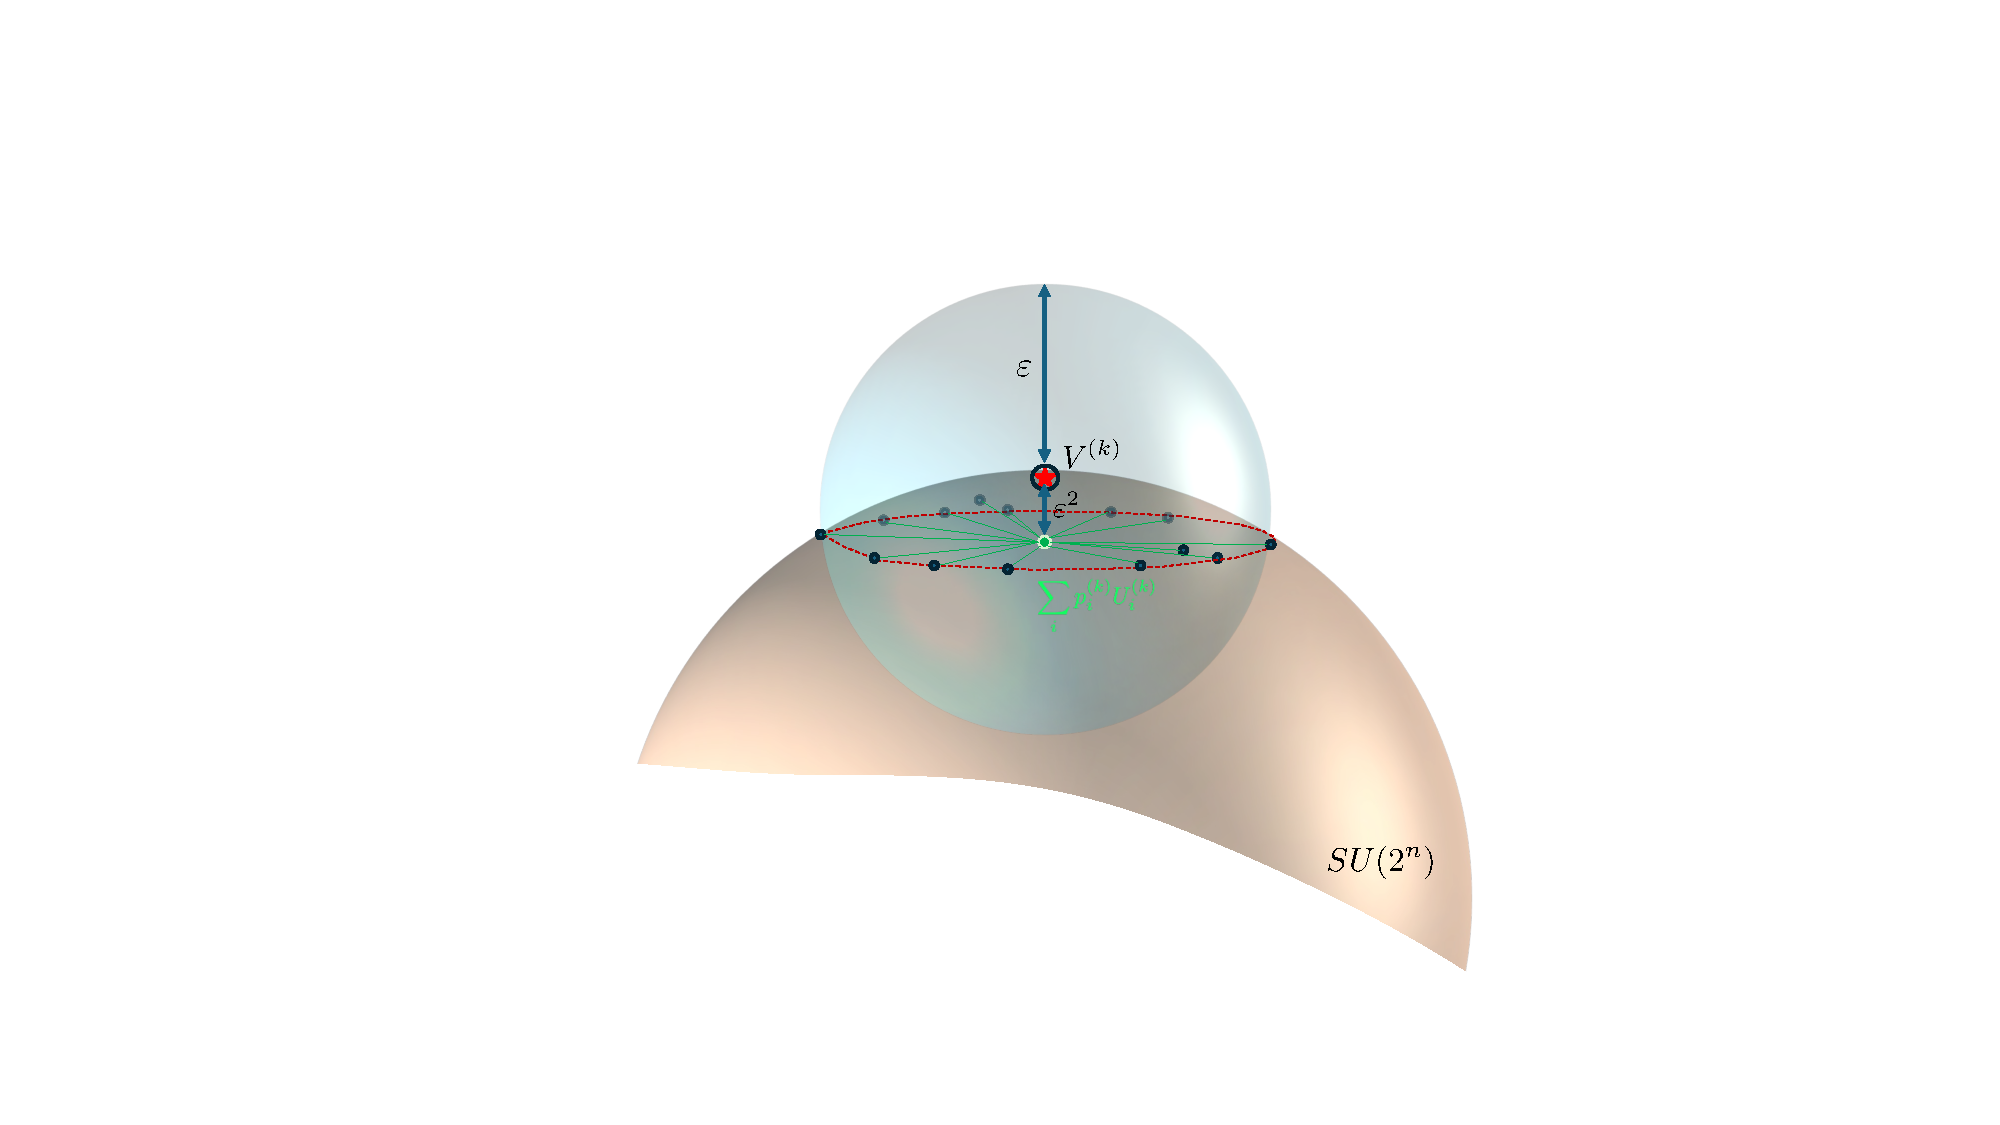
\includegraphics[width=0.8\linewidth]{figures/geometric.pdf}
\caption{
(a) Geometric intuition for the reduced Frobenius error condition. Ensemble members (blue dots) lie within an $\epsilon$-ball (light blue) around the target $V^{(k)}$ (red star). Their convex hull (dashed orange) contains the target, ensuring the weighted ensemble (green dot) lies within an $\epsilon^2$-ball (light green).
}
\label{fig:reduced_bias_combined}
\end{figure}


\begin{table*}[t]
\centering
\scriptsize
\resizebox{\textwidth}{!}{%
\begin{tabular}{|l|r|r|r|r|r|r|}
\hline
Circuit & Reference & $\epsilon^2 = 10^{-2}$ & $\epsilon^2 = 10^{-4}$ & $\epsilon^2 = 10^{-6}$ & $\epsilon^2 = 10^{-8}$ & $\epsilon^2 = 10^{-10}$ \\
\hline
Heisenberg-7q & 360 & \textbf{259.1 (-28.0\%)} & \textbf{296.5 (-17.6\%)} & \textbf{323.9 (-10.0\%)} & 332.9 (-7.5\%) & \textbf{322.1 (-10.5\%)} \\
\hline
Fermi Hubbard-8q & 91 & 84.9 (-6.7\%) & 84.0 (-7.7\%) & 85.0 (-6.6\%) & 82.9 (-8.9\%) & 91 (0\%) \\
\hline
QAOA-10q & 60 & \textbf{53.5 (-10.8\%)} & \textbf{52.5 (-12.5\%)} & 54.4 (-9.3\%) & \textbf{51.6 (-14.0\%)} & 55.5 (-7.5\%) \\
\hline
Li-H Sim-12q & 4555 & \textbf{3729.4 (-18.1\%)}  & 4403.5 (-3.3\%) & 4405.9 (-3.3\%) & 4412.2 (-3.1\%) & 4450.4 (-2.3\%) \\
\hline
QFT Add-12q & 96 & 96 (0\%) & 96 (0\%) & 96 (0\%) & 96 (0\%) & 96 (0\%) \\
\hline
QAE-13q & 156 & 155.7 (-0.2\%) & 155.8 (-0.1\%) & 156 (0\%) & 156 (0\%) & 156 (0\%) \\
\hline
QPE-14q & 3444 & 3444 (0\%) & 3444 (0\%) & 3444 (0\%) & 3444 (0\%) & 3444 (0\%) \\
\hline
Mult-16q & 1108 & \textbf{963.4 (-13.0\%)} & \textbf{944.3 (-14.8\%)} & 1008 (-8.9\%) & 1021.5 (-7.8\%) & 1083.4 (-2.3\%) \\
\hline
Lattice Sim-17q & 124 & \textbf{107.4 (-13.4\%)} & \textbf{110.6 (-10.8\%)} & \textbf{107.4 (-13.4\%)} & \textbf{107.6 (-13.2\%)} & \textbf{112.9 (-9.0\%)} \\
\hline
QAE-33q & 1026 & \textbf{610.3 (-40.5\%)} & \textbf{724.9 (-29.3\%)} & \textbf{915.7 (-10.7\%)} & 1026 (0\%) & 1026 (0\%) \\
\hline
QAOA-148q & 1752 & 1751.0 (-0.1\%) & 1751.0 (-0.1\%) & 1751.0 (-0.1\%) & 1751.0 (-0.1\%) & 1752 (0\%) \\
\hline
Lattice Sim-380q & 3026 & \textbf{2934.6 (-3.0\%)} & 2944.8 (-2.7\%) & 2943.7 (-2.7\%) & 2941.6 (-2.8\%) & 2985.8 (-1.3\%) \\
\hline
\end{tabular}
}
\caption{CNOT Reductions across our set of benchmarks for a range of output error ($\epsilon^2$) values. For our reference circuit, we show results after performing a full peephole optimization in PyTket \cite{tket}, a state of the art exact compilation tool. We run our workflow on this optimized circuit. Significant CNOT reductions $\geq 10\%$ are marked in bold.}
\label{tab:nisq}
\end{table*}

\begin{table*}[t]
\setlength{\tabcolsep}{5pt}
\centering
\scriptsize
\begin{tabular}{|l|r | r|r | r|r | r|r | r|r | r|}
\hline
\multirow{2}{*}{Circuit} 
& \multicolumn{2}{c|}{$\epsilon^2 = 10^{-2}$} 
& \multicolumn{2}{c|}{$\epsilon^2 = 10^{-4}$} 
& \multicolumn{2}{c|}{$\epsilon^2 = 10^{-6}$} 
& \multicolumn{2}{c|}{$\epsilon^2 = 10^{-8}$} 
& \multicolumn{2}{c|}{$\epsilon^2 = 10^{-10}$} \\
\cline{2-11}
& \textbf{Ref.} & \textbf{Ens.} & \textbf{Ref.} & \textbf{Ens.} & \textbf{Ref.} & \textbf{Ens.} & \textbf{Ref.} & \textbf{Ens.} & \textbf{Ref.} & \textbf{Ens.} \\
\hline
Heisenberg-7q 
& 7240 & \textbf{1602.3 (-78\%)} 
& 11120 & \textbf{4061.3 (-63\%)} 
& 14800 & \textbf{6828.0 (-54\%)} 
& 18440 & \textbf{8800.7 (-52\%)} 
& 21960 & \textbf{10779.1 (-51\%)} \\
\hline
Fermi Hubbard-8q 
& 1358 & \textbf{807.0 (-41\%)} 
& 2068 & \textbf{1321.1 (-36\%)} 
& 2762 & \textbf{1804.5 (-35\%)} 
& 3492 & \textbf{2273.9 (-35\%)} 
& 4218 & \textbf{2749.3 (-35\%)} \\
\hline
QAOA-10q 
& 1180 & \textbf{565.3 (-52\%)} 
& 1840 & \textbf{954.2 (-48\%)} 
& 2386 & \textbf{1297.5 (-46\%)} 
& 3052 & \textbf{1683.2 (-45\%)} 
& 3650 & \textbf{2039.2 (-44\%)} \\
\hline
Li-H Sim-12q 
& 27570 & \textbf{20298.5 (-26\%)} 
& 44834 & \textbf{33119.9 (-26\%)} 
& 60076 & \textbf{44556.4 (-26\%)} 
& 76330 & \textbf{58768.0 (-23\%)} 
& 92204 & \textbf{71504.1 (-22\%)} \\
\hline
QFT Add-12q 
& 2879 & \textbf{2009.7 (-30.2\%)} 
& 4199 & \textbf{2737.3 (-34.8\%)} 
& 5725 & \textbf{3432.7 (-40.0\%)} 
& 6993 & \textbf{4612.7 (-34.0\%)} 
& 8543 & \textbf{6115.8 (-28.4\%)} \\
\hline
QAE-13q 
& 6339 & \textbf{3337.4 (-47\%)} 
& 9471 & \textbf{5166.4 (-45\%)} 
& 12637 & \textbf{7389.9 (-42\%)} 
& 15647 & \textbf{9699.6 (-38\%)} 
& 18953 & \textbf{13502.8 (-29\%)} \\
\hline
QPE-14q 
& 126100 & 121870.4 (-3\%) 
& 187450 & 179895.5 (-4\%) 
& 250954 & 238468.1 (-5\%) 
& 312372 & 294709.0 (-6\%) 
& 373568 & 351661.5 (-6\%) \\
\hline
Mult-16q 
& 43126 & 39583.3 (-8\%) 
& 63906 & \textbf{49069.6 (-23\%)} 
& 86372 & \textbf{60497.5 (-30\%)} 
& 106016 & 90447.7 (-15\%)
& 128880 & 119441.3 (-7\%) \\
\hline
Latt. Sim-17q 
& 3806 & \textbf{2514.6 (-34\%)} 
& 6086 & \textbf{4111.3 (-32\%)} 
& 7874 & \textbf{5433.0 (-31\%)} 
& 9906 & \textbf{6765.0 (-32\%)} 
& 12136 & \textbf{8434.1 (-31\%)} \\
\hline
QAE-33q 
& 31842 & \textbf{25444.7 (-20\%)} 
& 56840 & 46367.2 (-18\%) 
& 81828 & 70327.7 (-14\%) 
& 101446 & 87478.6 (-14\%) 
& 122258 & 103978.1 (-15\%) \\
\hline
QAOA-148q 
& 47440 & \textbf{34612.4 (-27\%)} 
& 72750 & \textbf{39842.4 (-45\%)} 
& 100146 & 81231.7 (-19\%) 
& 126206 & \textbf{90374.3 (-28\%)} 
& 152652 & \textbf{108960.3 (-29\%)} \\
\hline
Lattice Sim-380q 
& 85686 & 76452.8 (-11\%) 
& 138560 & 126252.6 (-9\%) 
& 179604 & \textbf{130030.8 (-28\%)} 
& 226730 & 194379.3 (-14\%) 
& 277804 & 242570.8 (-13\%) \\
\hline
\end{tabular}
\caption{T gate reductions across our set of benchmarks for a range of output error ($\epsilon^2$) values. The reference circuit is generated with a PyTket optimized circuit for which all $R_z$ gates are approximately compiled into a fixed gateset by Gridsynth to error $\epsilon^2$. Significant T gate reductions $\geq 20\%$ are marked in bold.}
\label{tab:ft}
\end{table*}


\subsection*{Demonstration of resource reduction with controlled output error}
\label{sec:demos}
In the following, we demonstrate gate count reduction while controlling output error for a diverse set of benchmarks, including key quantum subroutines (Adders, Mults, QAEs, and Modular Exponentiation), Hamiltonian simulations (LiH, Fermi-Hubbard, Heisenberg, and Lattice Gauge Simulation), and optimization algorithms (QAOA). The circuit widths for these benchmarks vary from 7 qubits to 380 qubits. See Supplementary Information (SI), Section 1, for more details on each of the benchmarks. The implementations of the components in the workflow, Fig. \ref{fig:resut_workflow}, are discussed in Methods. 
For NISQ architectures, we compile to CNOT and arbitrary single-qubit gates, minimizing CNOT count. For FT architectures, we compile to single-qubit Clifford, CNOT, and $R_z$ gates, and then use Gridsynth \cite{ross_sellinger} to approximate the $R_z$ rotations as a sequence of $H, S$ and $T$ gates. We compare performance against \emph{optimized} reference circuits that are generated using PyTKet \cite{tket} with full peephole optimization. For the FT case, PyTKet compiles and optimizes into Clifford and $R_z$ gates and we again use Gridsynth to approximate the $R_z$ rotations. Note that while in the NISQ case, we compare against a reference circuit that exactly implements the target unitary, in the FT setting the reference is also an approximate circuit. In order to have fair comparison, in our workflow we use Gridsynth to synthesize each $R_z$ gate in a circuit with $n_Z$ $R_z$ gates to error $\frac{\epsilon}{n_Z}$, whereas in the reference each $R_z$ gate is synthesized to error $\frac{\epsilon^2}{n_Z}$. This ensures that the overall circuit/channel error is $O(\epsilon^2)$ in both cases. Unless otherwise stated, all numerical demonstrations use partitions consisting of subcircuits acting on four qubits; the rationale for this choice is discussed in the Methods section.

Tables \ref{tab:nisq} and \ref{tab:ft} summarize the gate count reductions achieved by our workflow for the benchmark suite.  
Table \ref{tab:nisq} reports CNOT counts for the exact (reference) compilation and the average CNOT counts for the circuit ensembles generated by our workflow for various output error bounds $\epsilon^2$.  
In most cases, we achieve reductions over the exact compilation, in some instances significantly (marked in bold). There are, however, notable exceptions. In the NISQ case, we see no improvement for the Multiplier, Fermi Hubbard, QPE, and QFT Adder circuits. In these cases, the exactly optimized circuits produce circuits with an extremely "rigid" structure. Across all blocks, our synthesis techniques were unable to find significant CNOT reductions while maintaining low approximation errors. As we reduced our error budget, our synthesizer would only find one or two reduced circuits. While these circuits did have fewer CNOTs, they were not sufficient to quadratically reduce the weighted ensemble error. We provide examples of such blocks in the SI, Section 2. 

Table \ref{tab:ft} presents results for the FT workflow.  
Here, we report $T$-gate counts for both the reference and our workflow, for various target output error values. Our approach reduces $T$-gate counts for all benchmarks and all target error values. This is primarily because we can leverage a higher approximation error for $R_z$ synthesis than the reference compilation.

Having demonstrated resource reductions, we now show that our approach also controls the output error of the compiled circuits. 
Direct numerical calculation of the diamond distance between the channel output by our approach and the ideal circuit is infeasible for our benchmarks. Instead, we use the fact that the diamond distance upper bounds both observable errors and output state errors, and we evaluate these more tractable quantities.

Figure \ref{fig:obs_scaling} shows the observable error for three benchmark applications where observable measurement is appropriate.  
For each benchmark, we compute the expected value of an observable using the ideal circuit unitary, denoted $O_{\mathrm{ideal}}$ (the specific observables for each benchmark are described in the SI, Section 1).  
We then compute the same observable using the channel induced by the ensemble of compiled circuits produced by our workflow, for a range of target errors,  $O_{\mathrm{ens}} = \sum_{p_i \in \mathbb{P}} p_i O(U_i)$,
where $p_i$ are the probabilities assigned to circuits $U_i$ in the ensemble, the blocks of each $U_i$ are synthesized to Frobenius norm error $\epsilon$, and $O(U_i)\equiv\bra{\psi_0}U_i\dg O U_i \ket{\psi_0}$.  
To isolate the effects of compilation error, we neglect shot noise in both $O_{\mathrm{ideal}}$ and $O_{\mathrm{ens}}$.  
We expect the observable error $|O_{\mathrm{ideal}} - O_{\mathrm{ens}}|$ to scale as $O(K\epsilon^2)$, where $K$ is the number of blocks in the partitioning of the input circuit.  
Indeed, Fig. \ref{fig:obs_scaling} confirms this scaling for both NISQ and FT compilation workflows.

\begin{figure*}[ht]
    \centering
    \begin{subfigure}{0.49\textwidth}
        \centering
        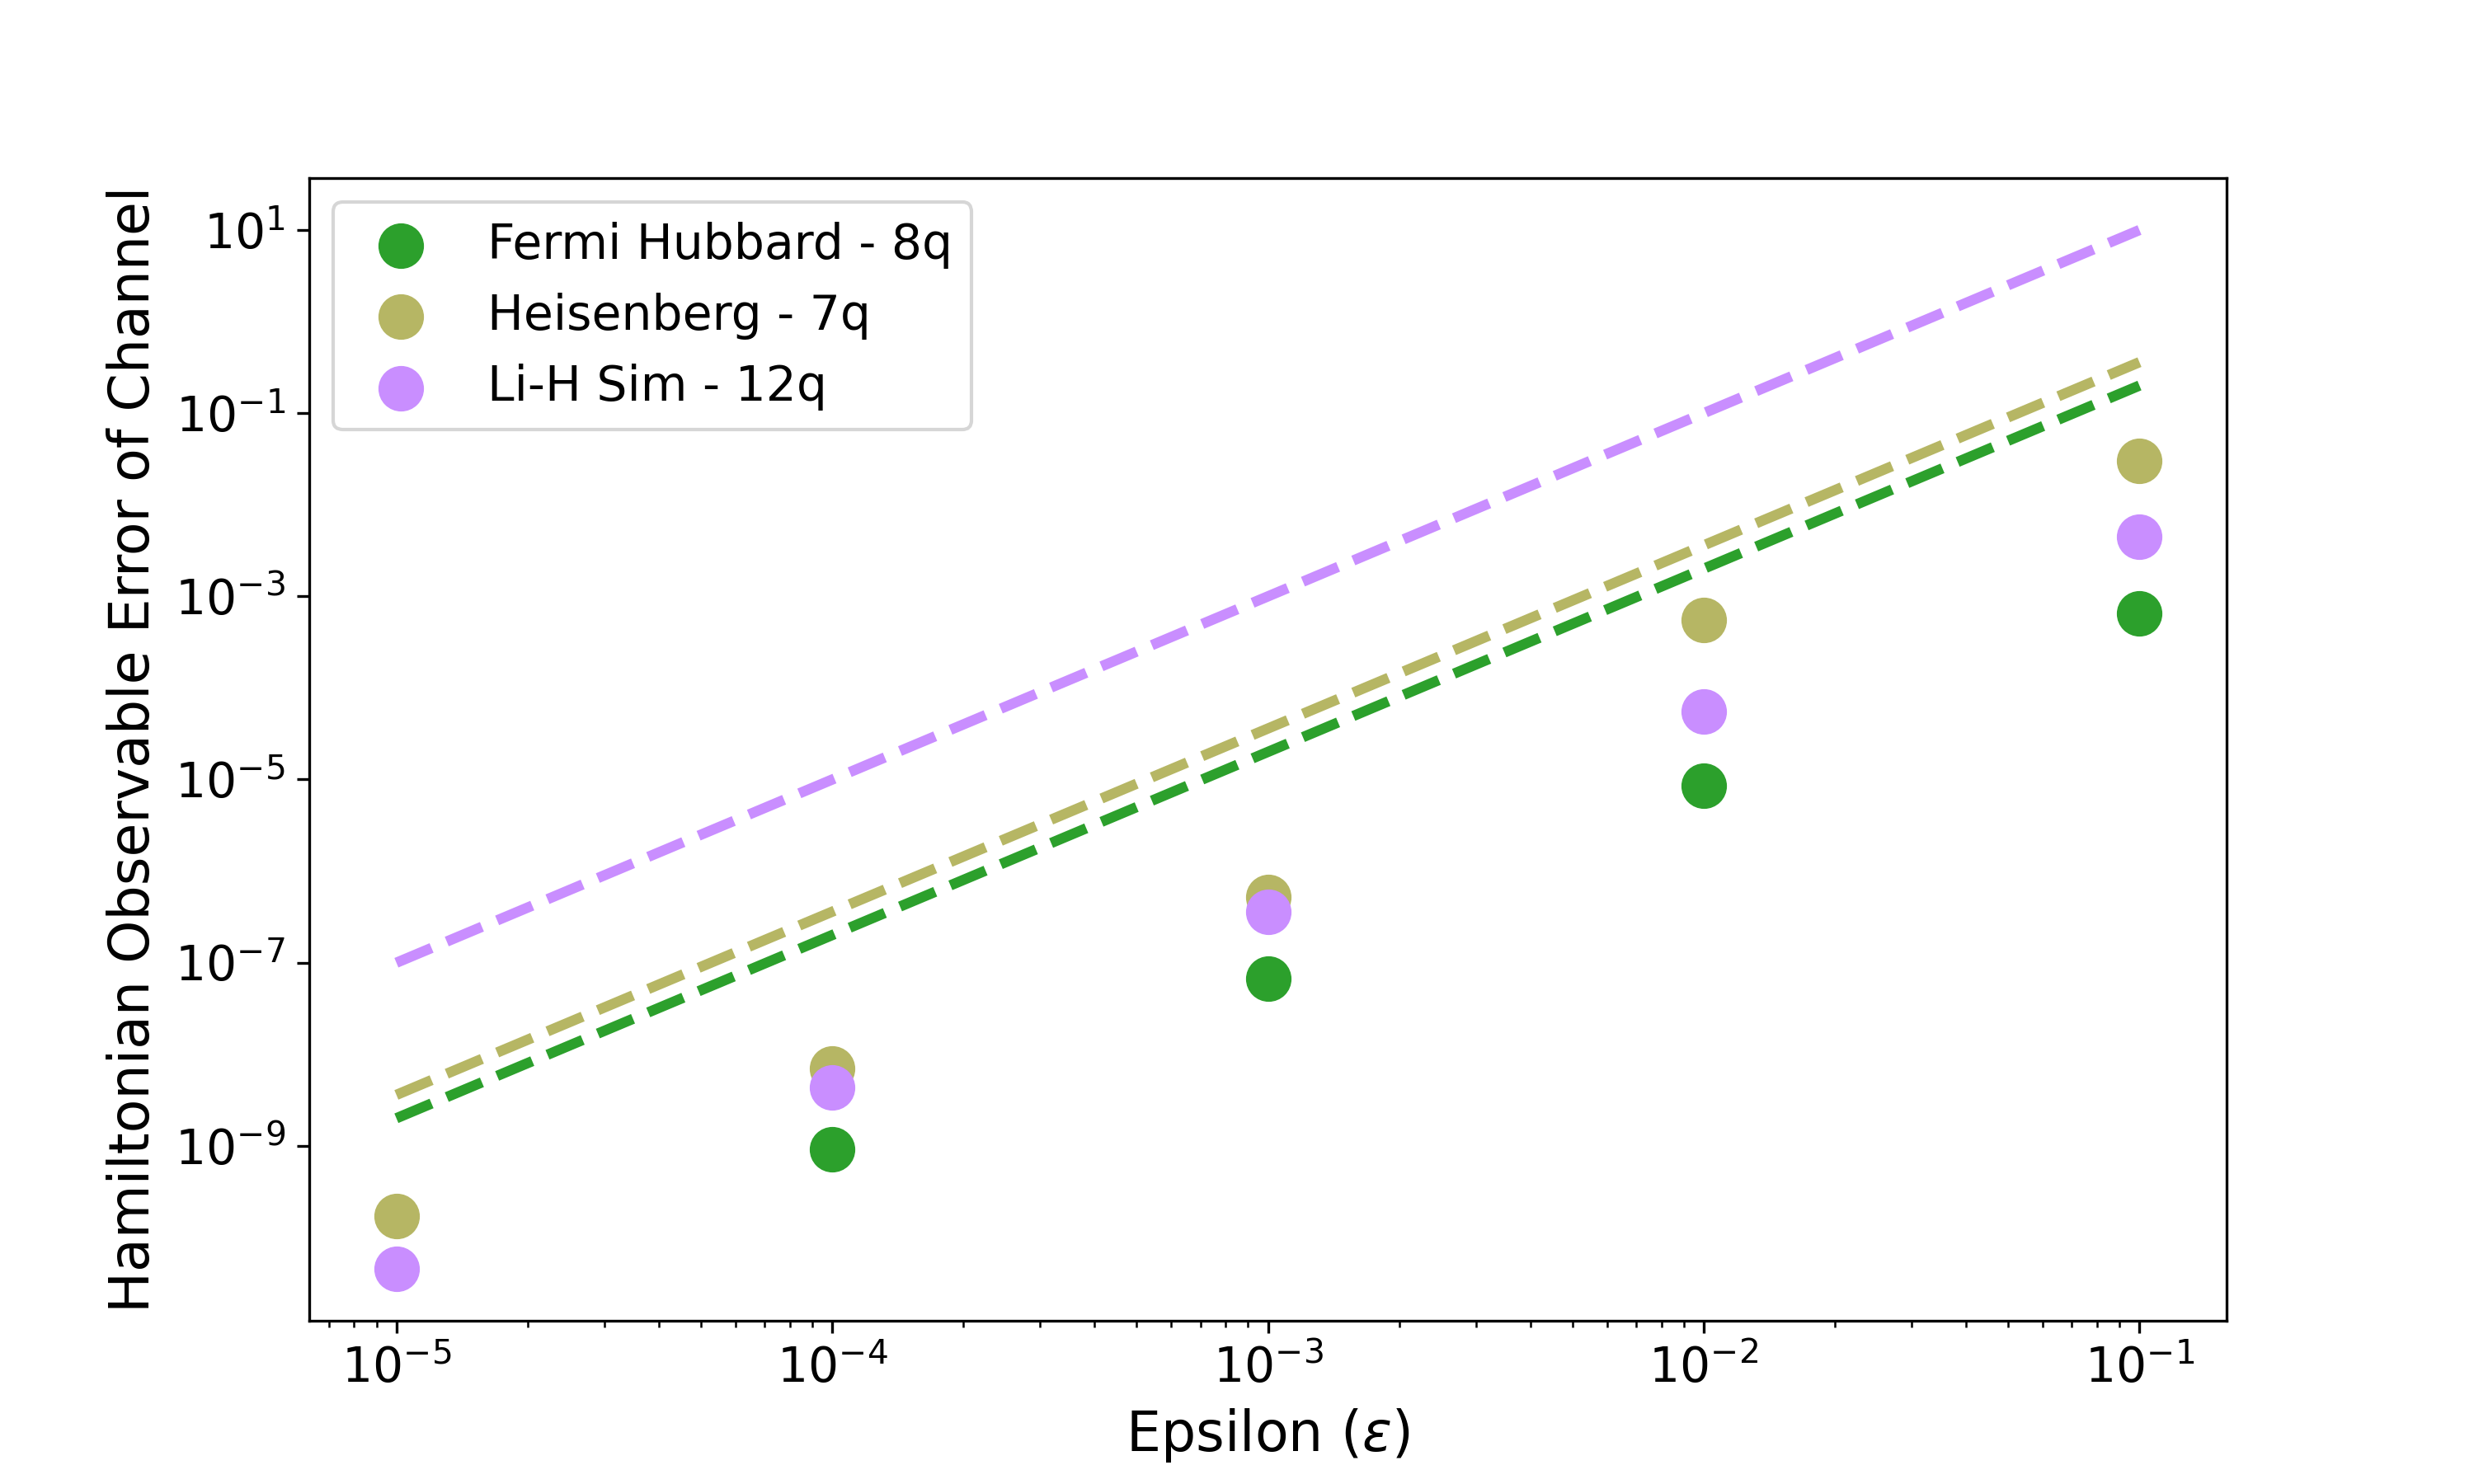
\includegraphics[width=\linewidth]{figures/hamiltonian_scaling_final.png}
    \end{subfigure}
    \begin{subfigure}{0.49\textwidth}
        \centering
        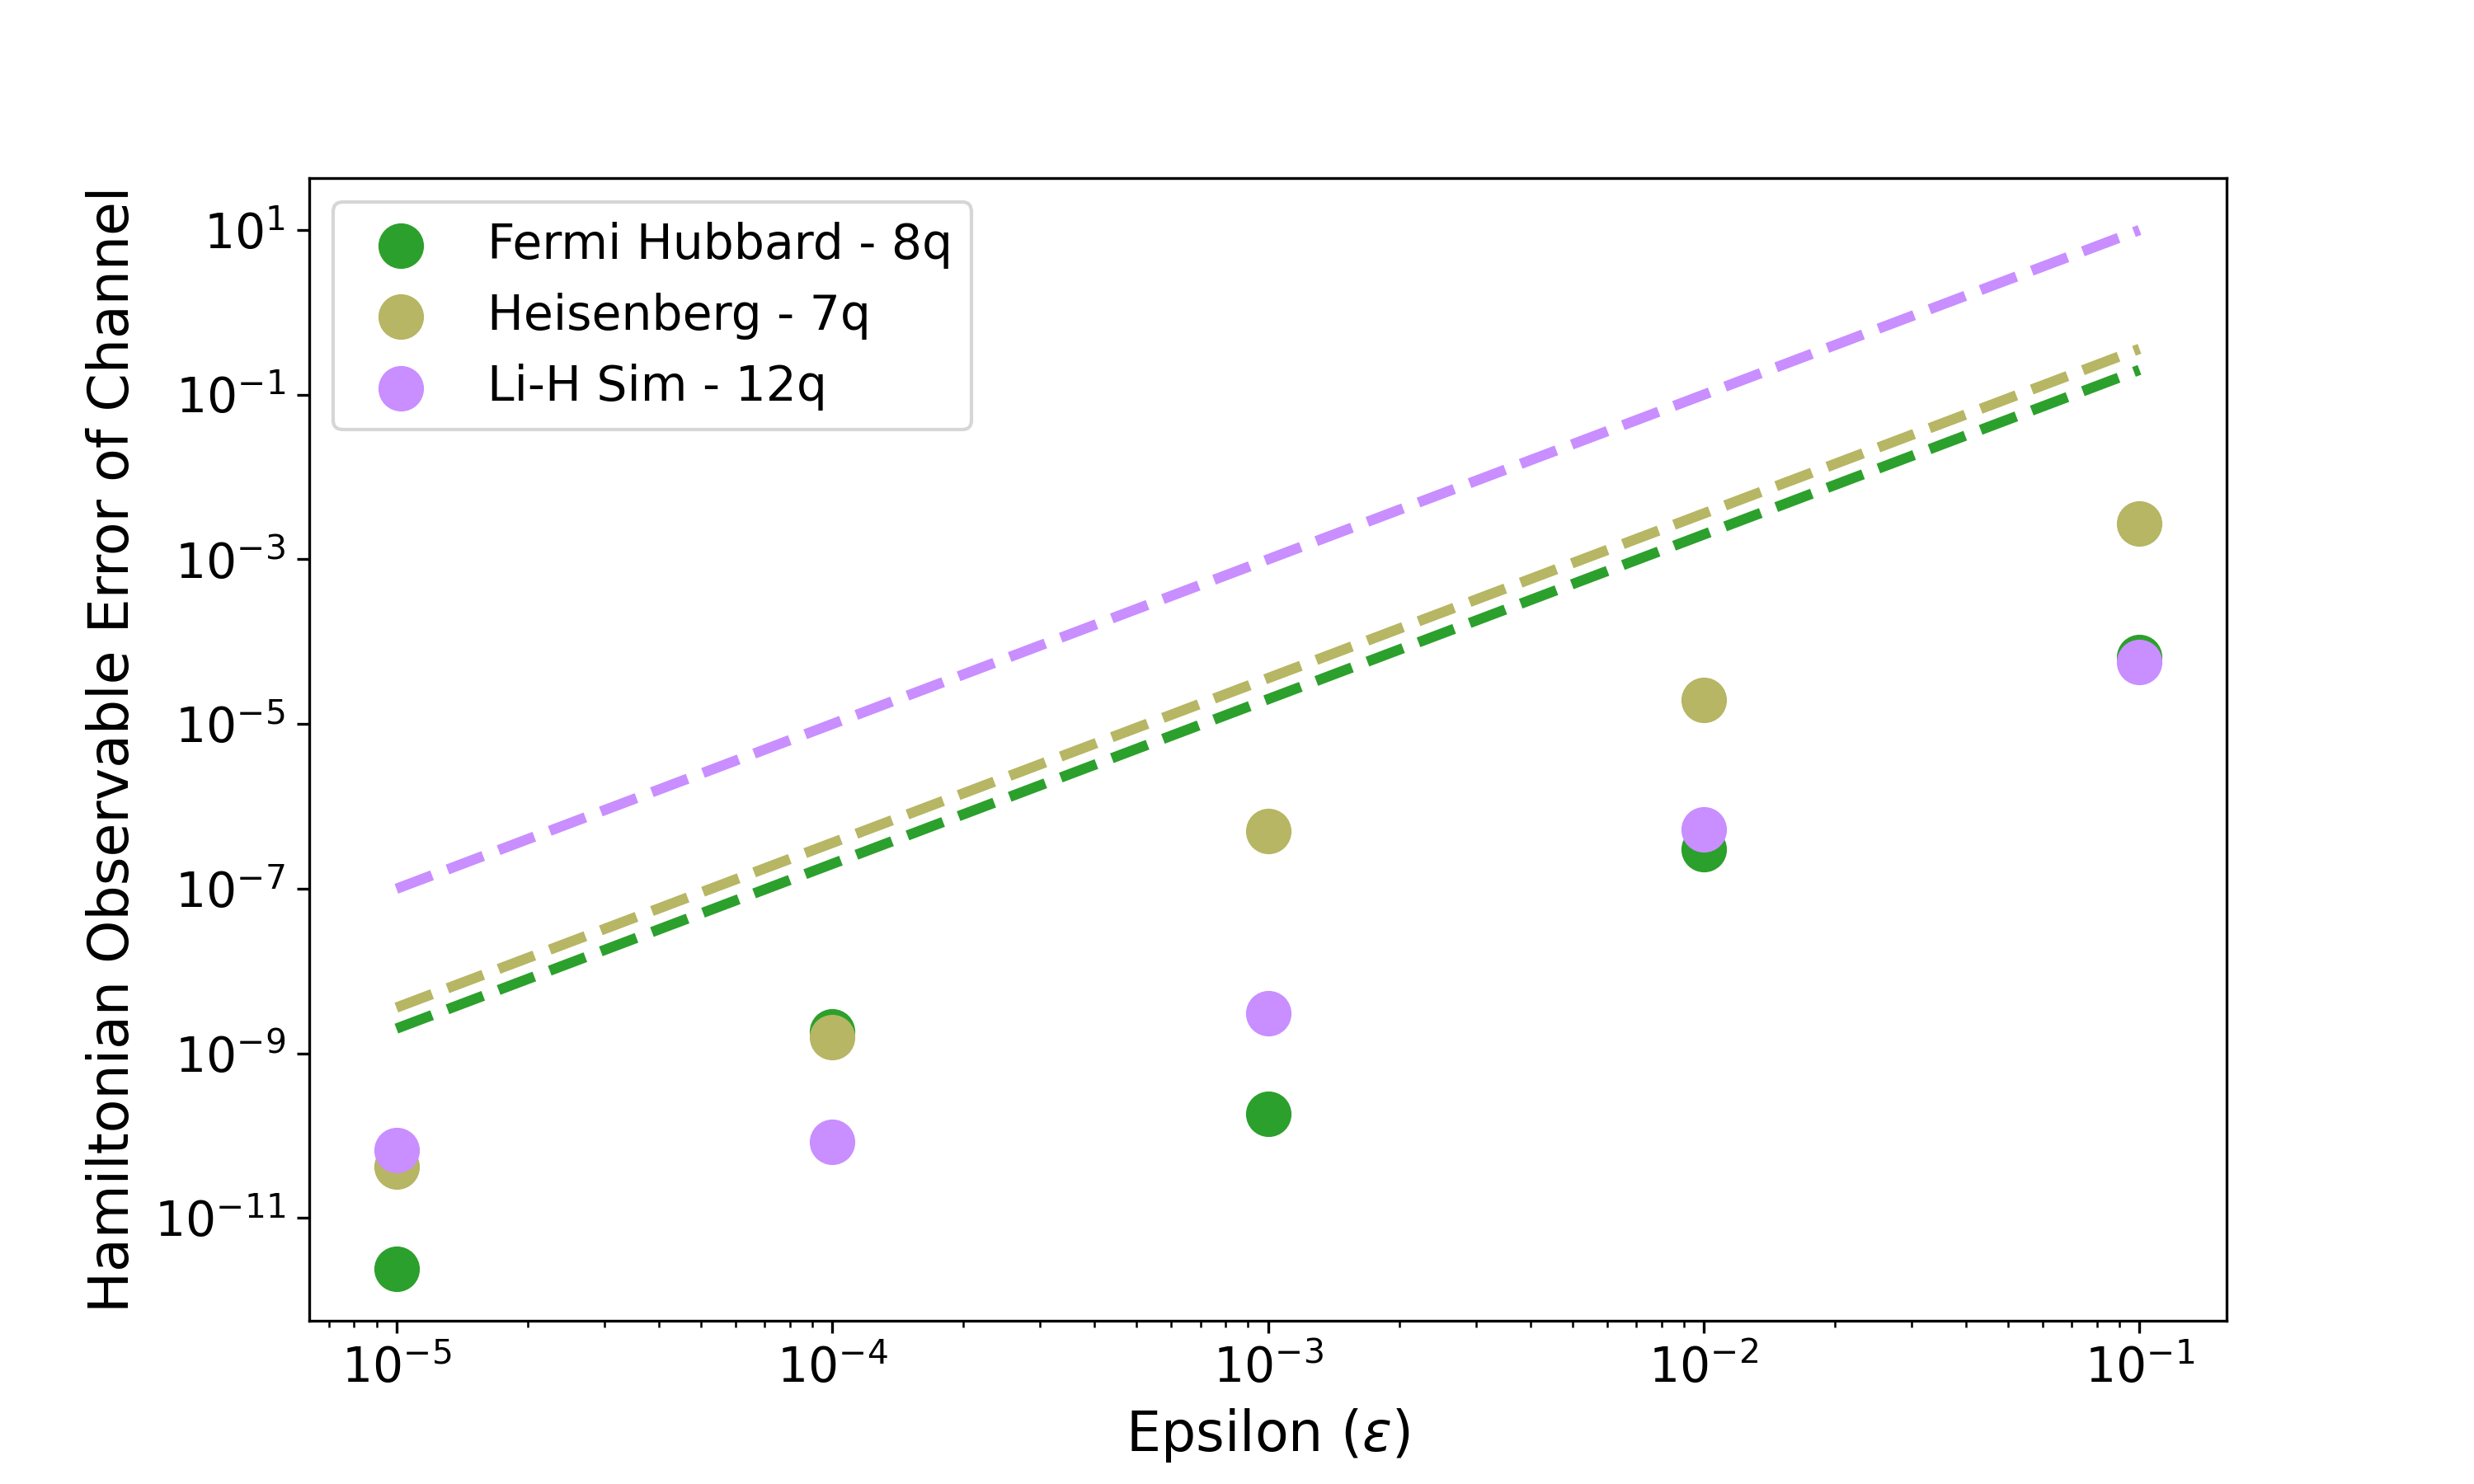
\includegraphics[width=\linewidth]{figures/hamiltonian_scaling_clifft_final_20.png}
    \end{subfigure} \\
    \caption{Observable errors (y-axis) for Fermi–Hubbard Model, LiH and Heisenberg benchmarks, as a function of the compilation error tolerance $\epsilon$.  
    The left panel shows NISQ compilation results; the right panel shows FT compilation results. For each benchmark, we draw a corresponding dotted line at $K\epsilon^2$ where $K$ is the number of blocks in the benchmark. Across all benchmarks, the observable error is bounded by this line.}
    \label{fig:obs_scaling}
\end{figure*}

An alternative error metric that is tractable to compute is the trace distance between the output state of the ensemble and the ideal output state for a given input state, $\frac{1}{2}\left\| \rho_{\mathrm{ens}} - \ket{\psi_{\mathrm{ideal}}}\bra{\psi_{\mathrm{ideal}}} \right\|_1$,
which upper bounds the error of any observable for that fixed input state.  
For each benchmark, we prepare a set of 10 random input density matrices and compute the corresponding output density matrices after applying the ensemble channel. We take the maximum trace distance over these random inputs as a proxy for the worst-case channel error, which cannot be computed exactly. Figure \ref{fig:trace_distance_scaling} shows that this proxy also scales as $O(K\epsilon^2)$ for both NISQ and FT workflows.

For a comprehensive picture of the error scaling our framework achieves, see the SI, Section 3, where we present statistics of the weighted ensemble error and ensemble bias across all blocks for all benchmarks.

\begin{figure*}[ht]
    \centering
    \begin{subfigure}{0.48\textwidth}
        \centering
        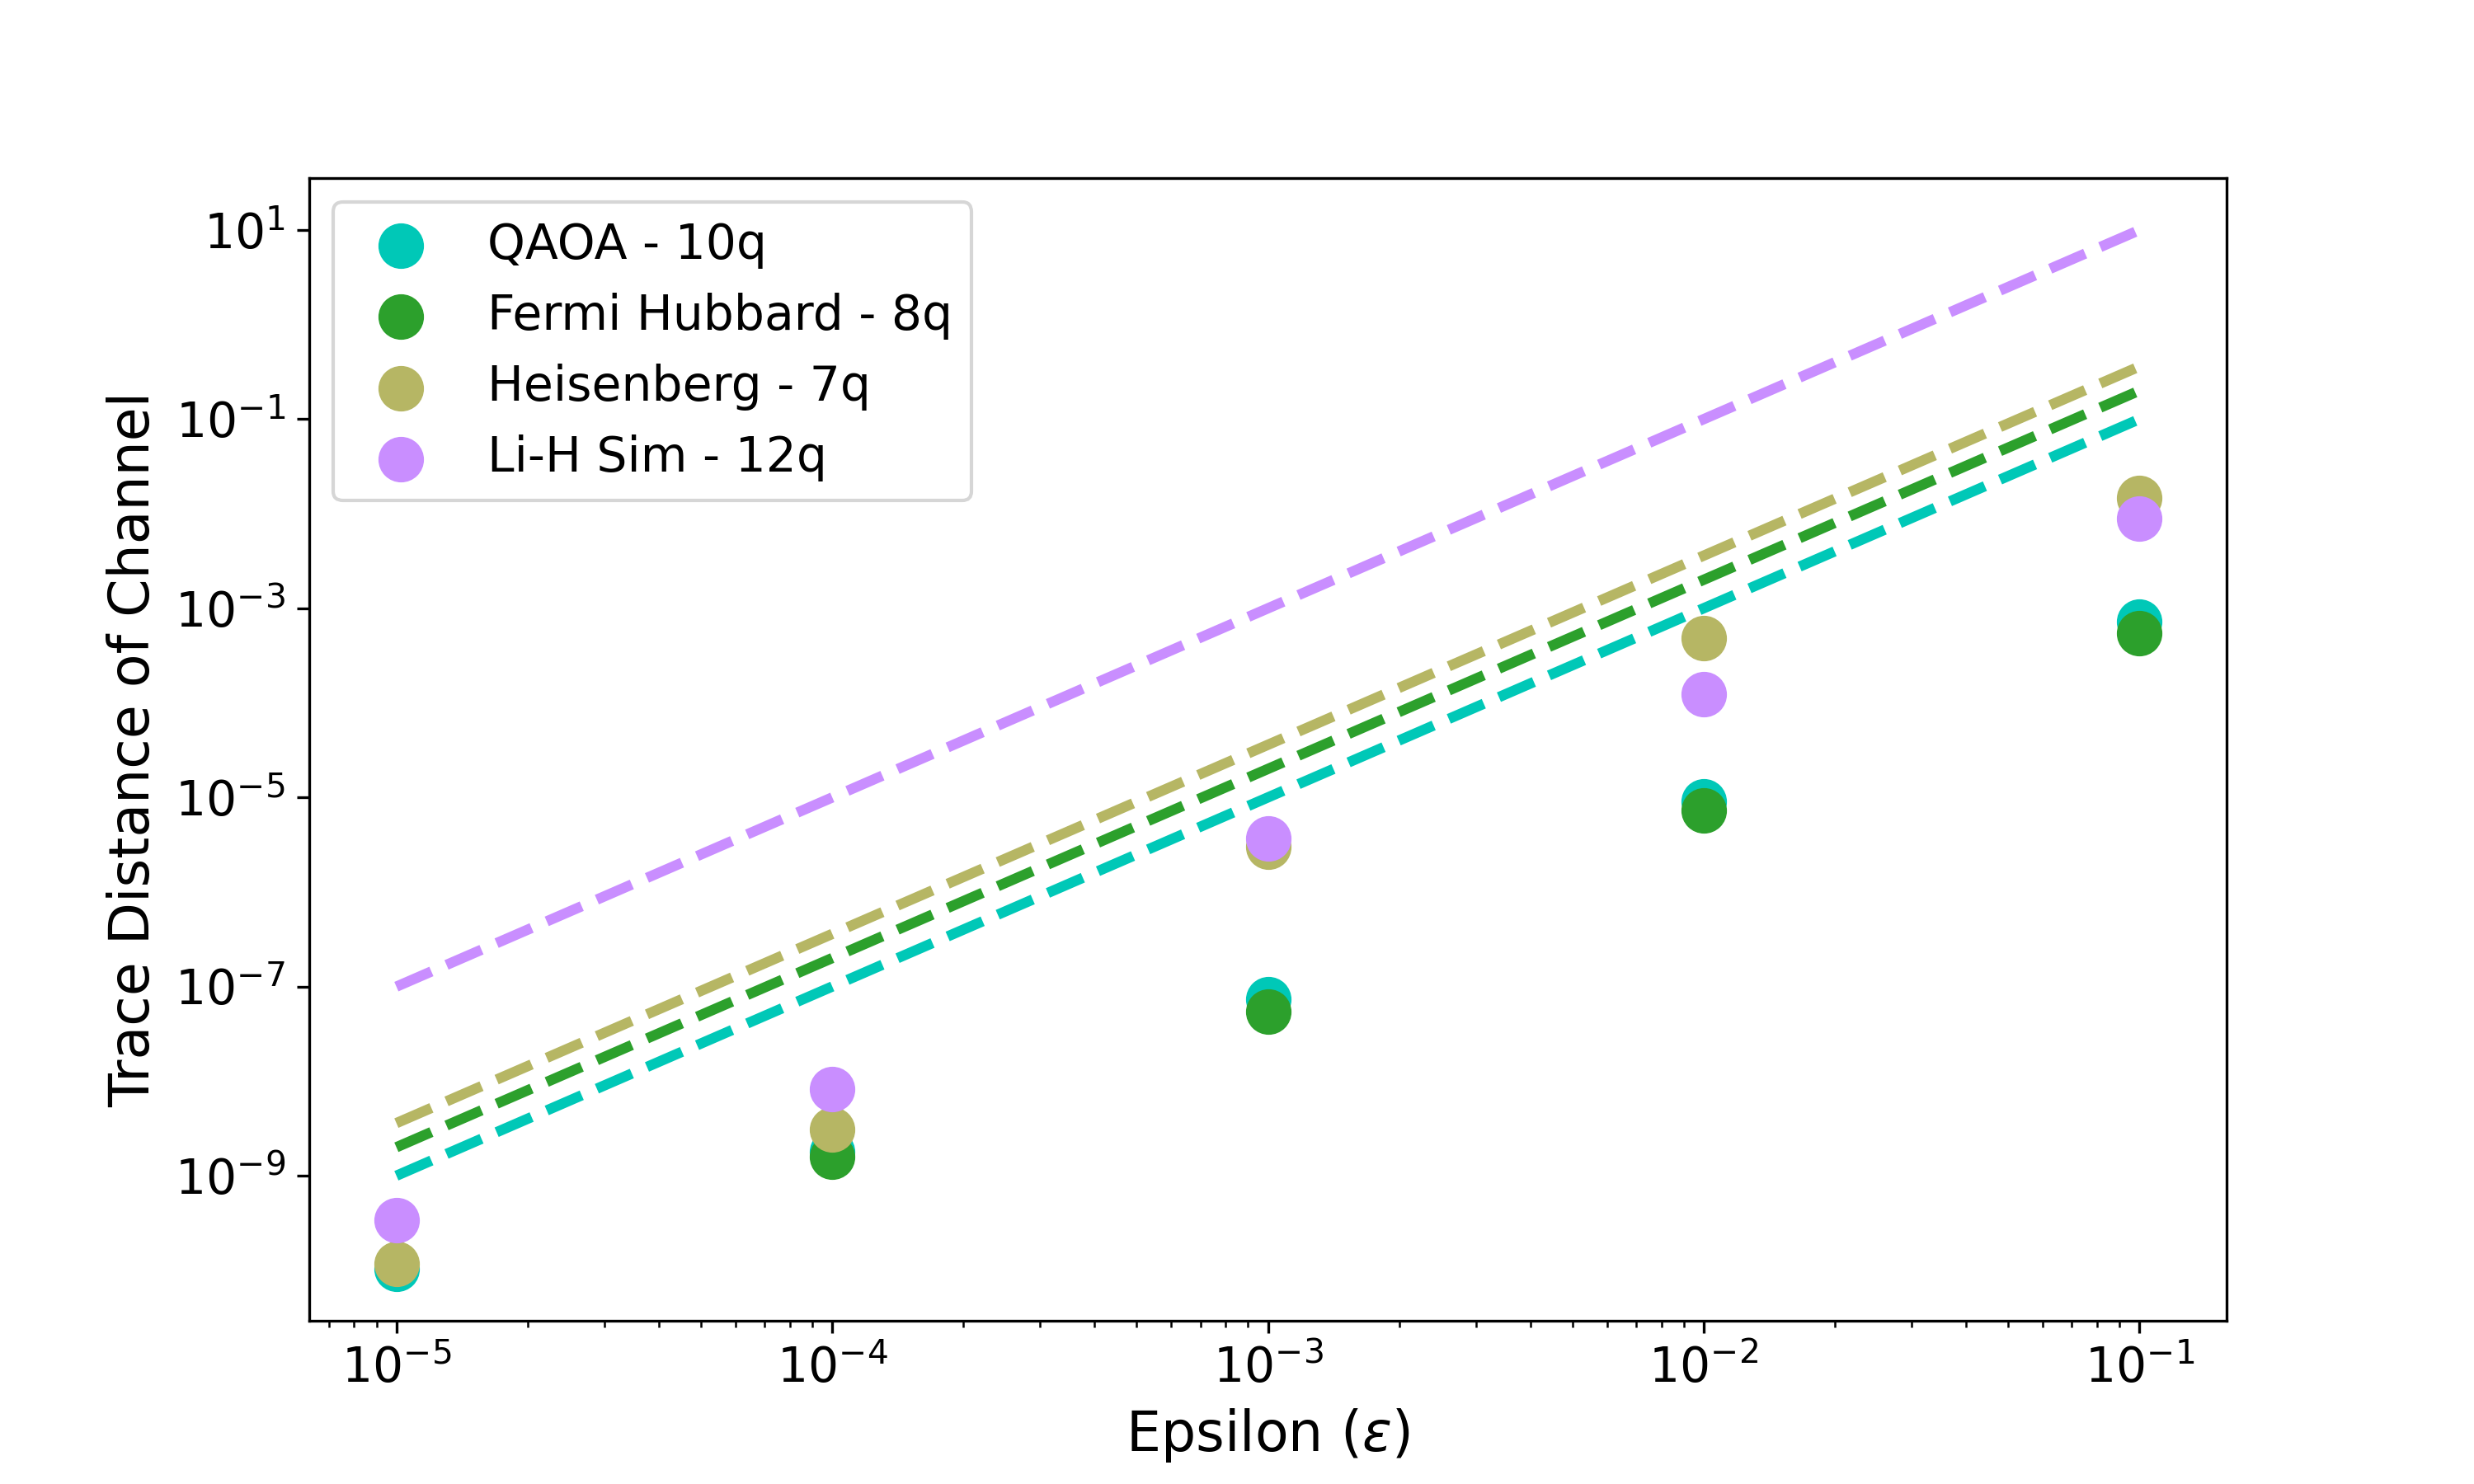
\includegraphics[width=\linewidth]{figures/trace_distance_scaling_final.png}
    \end{subfigure}
    \begin{subfigure}{0.48\textwidth}
        \centering
        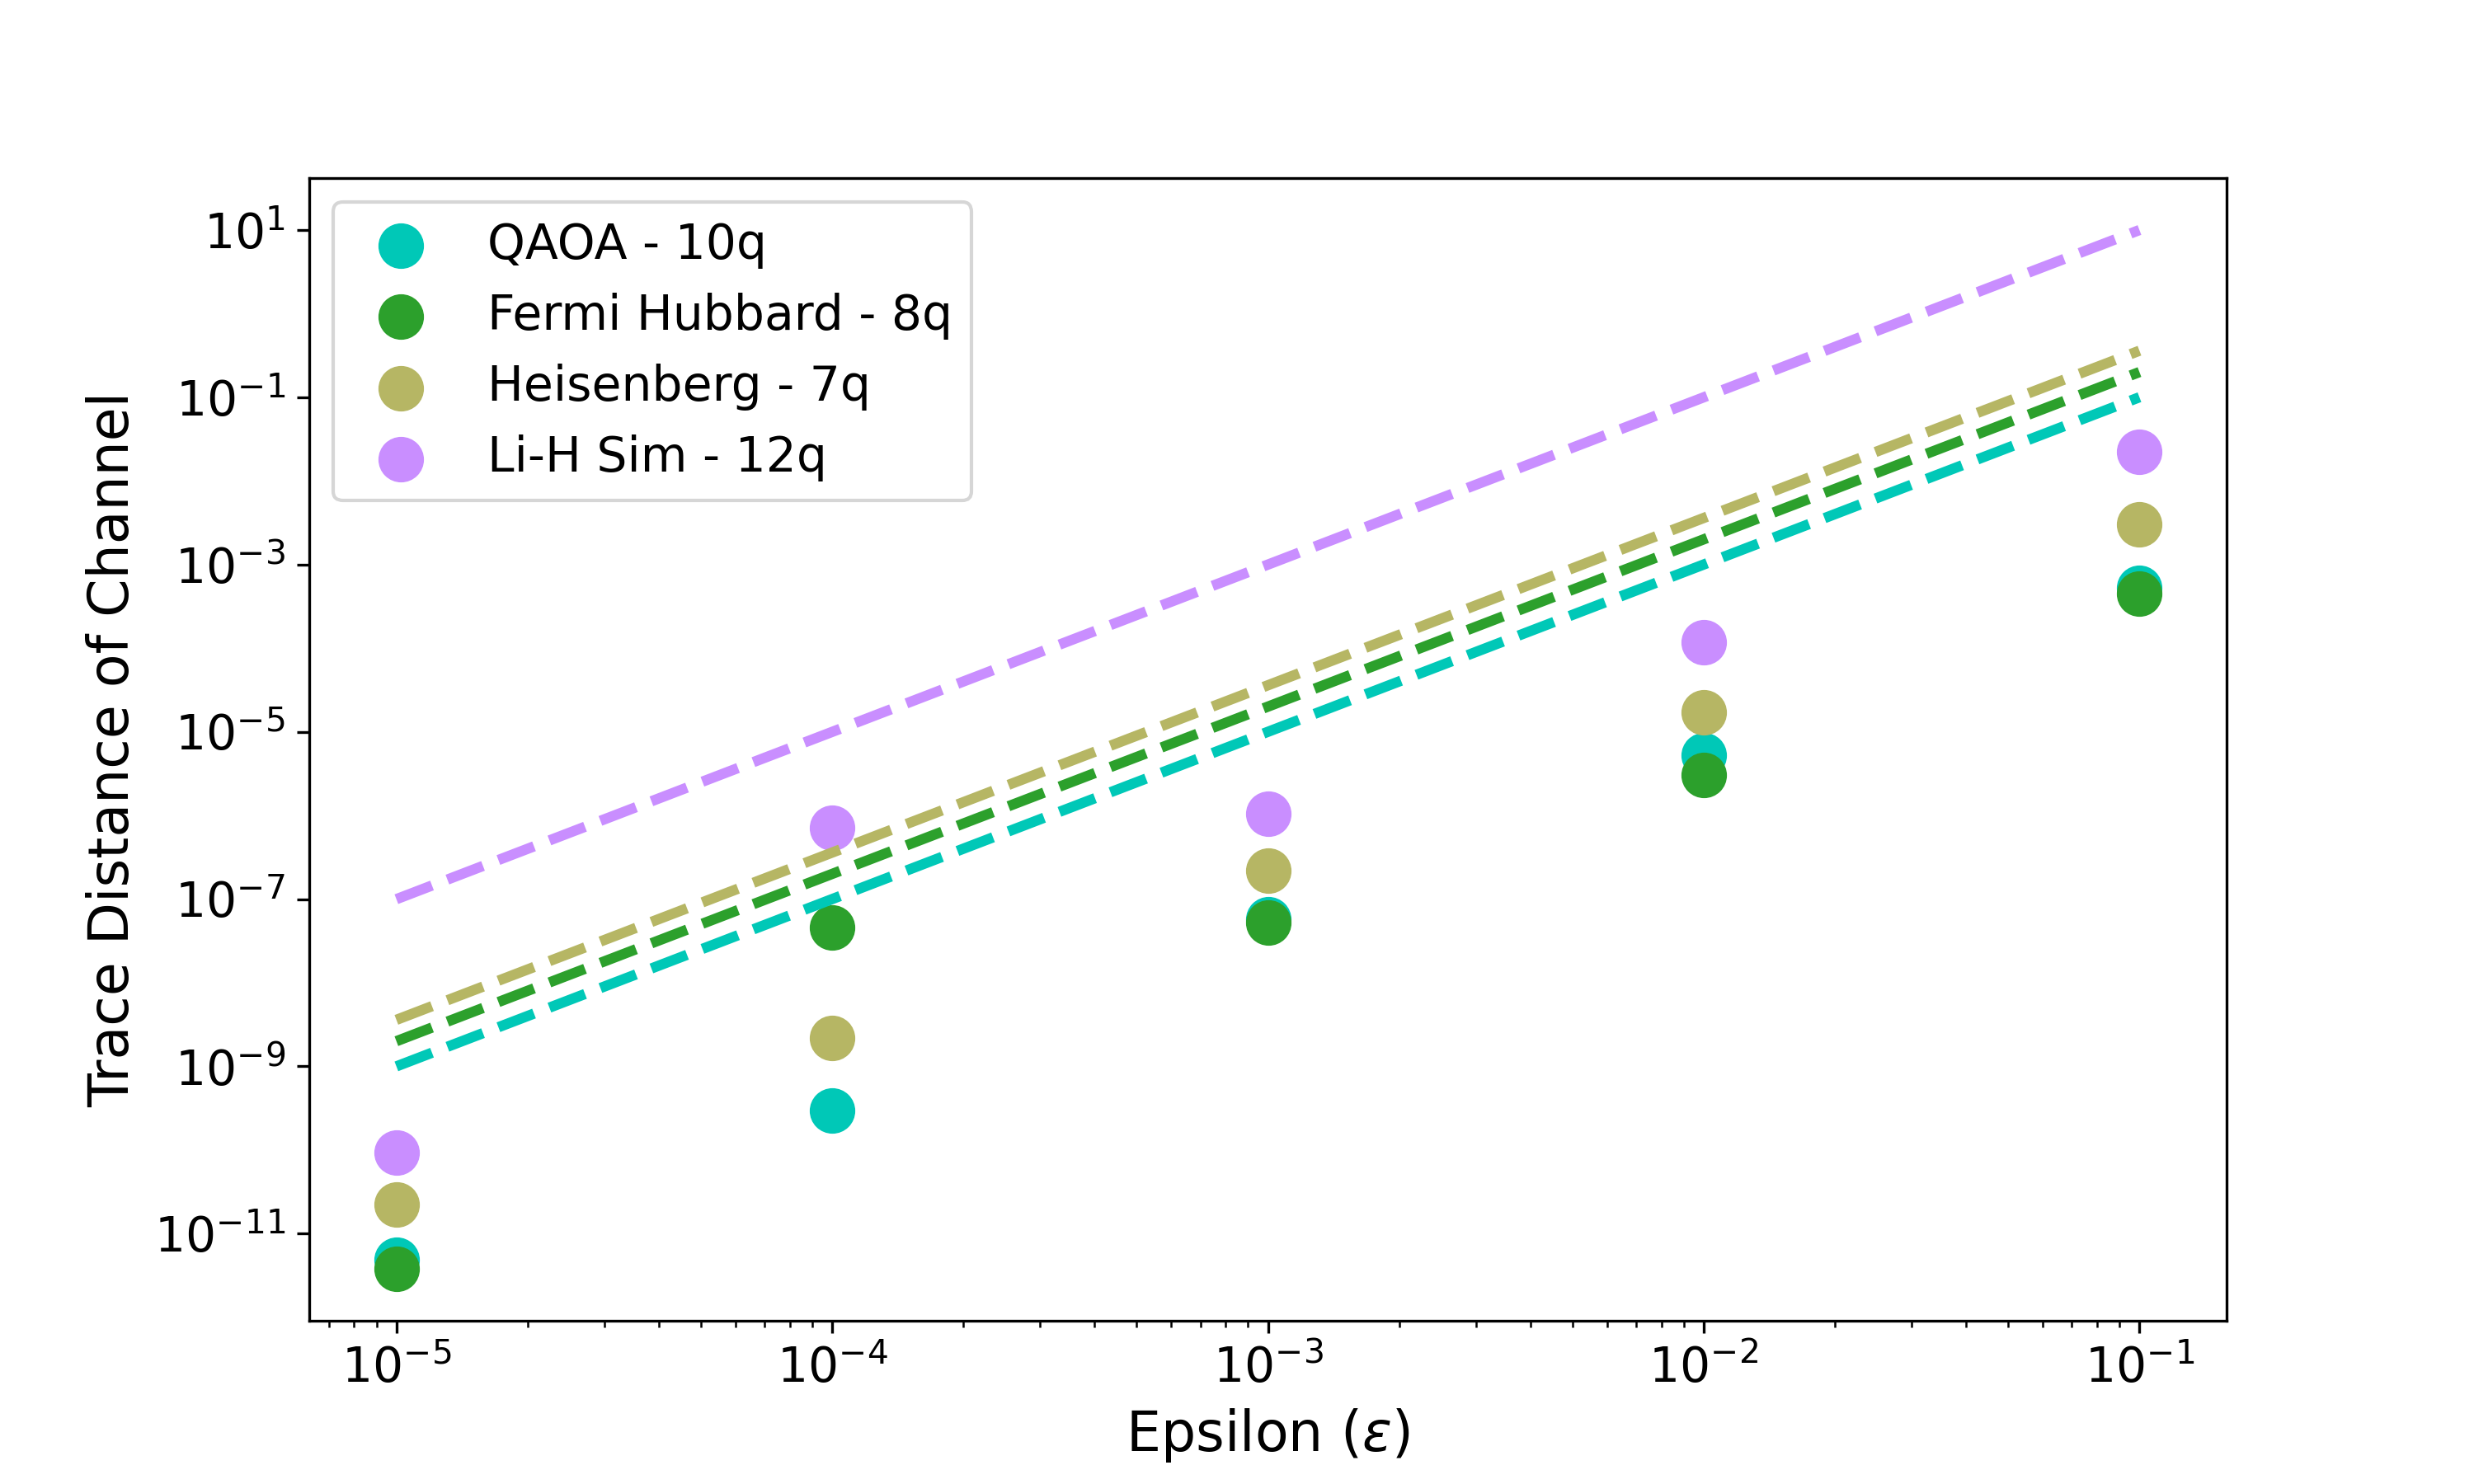
\includegraphics[width=\linewidth]{figures/trace_distance_scaling_clifft_final_20.png}
    \end{subfigure} \\
    \caption{Output state errors (y-axis) for the QAOA, Fermi Hubbard, Heisenberg, and LiH benchmarks. For each benchmark and each $\epsilon$, we generate a set of 10 random input density matrices and choose the density matrix that maximizes the output trace distance with respect to the original circuit. This metric serves as a proxy for the worst-case distance (diamond distance) which is intractable to solve. We plot this maximum trace distance (y-axis) between ensemble and ideal outputs as a function of $\epsilon$ (x-axis). The left panel shows NISQ results; the right shows FT results. For each benchmark, we draw a corresponding dotted line at $K\epsilon^2$ where $K$ is the number of blocks in the benchmark.
    In all cases, the trace distance is bounded by this line.}
    \label{fig:trace_distance_scaling}
\end{figure*}

\begin{figure}[ht!]
    \centering
    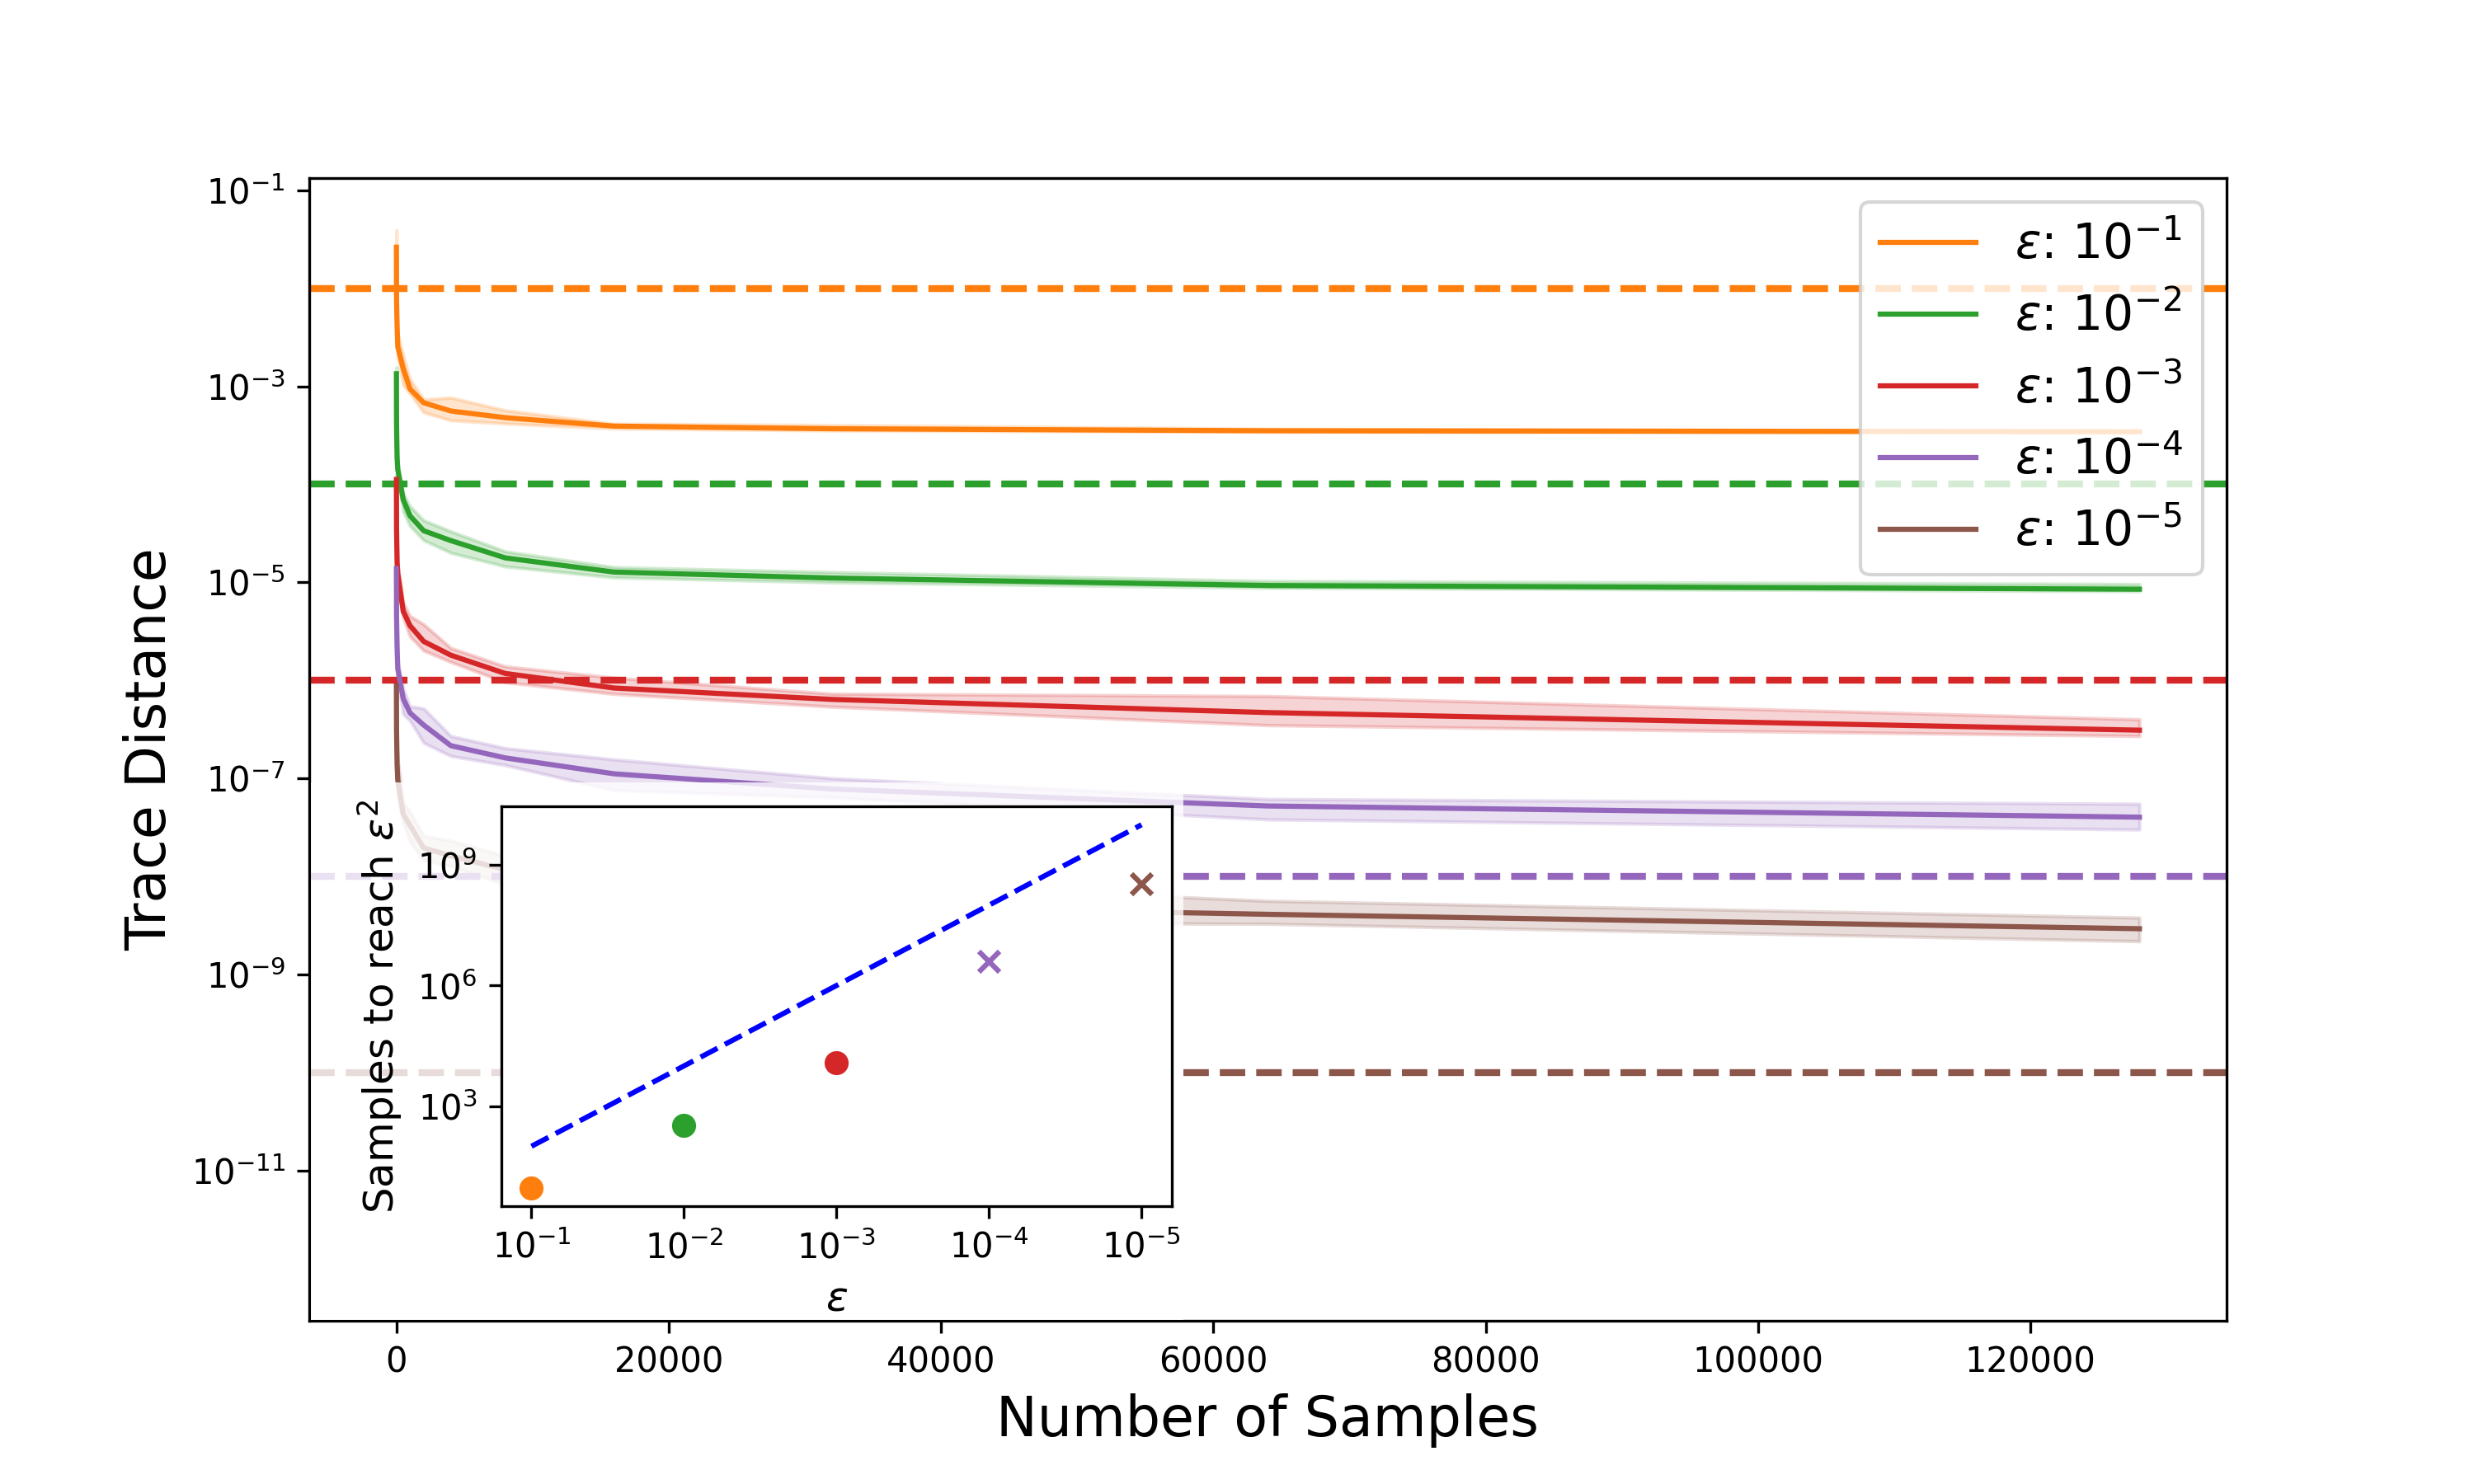
\includegraphics[width=1\linewidth]{figures/td_convergence_heisenberg7_final.png}
    \caption{Convergence of output state error, as measured by trace distance, for the 7-qubit Heisenberg benchmark as a function of the number of samples drawn from the ensemble channel.  Dotted horizontal lines indicate $\epsilon^2$ for each target $\epsilon$. We run 10 different trials at each sample and plot the average (solid line) as well as the full range (area). The inset figure plots the number of samples required until the sampled empirical channel, $\hat{\mathcal{U}}[\rho]$, achieves an average output state error $\epsilon^2$ from the true channel, $\mathcal{V}[\rho]$. The number of samples required for $\epsilon \in \{ 10^{-4}, 10^{-5} \}$ are extrapolated values. The dotted blue line is equal to $\epsilon^{-2}$, and empirically upper bounds the number of samples required.
    }
    \label{fig:td_convergences}
\end{figure}

\subsection*{Sample convergence of approximate ensembles}

An important practical consideration is the \emph{sample complexity}—the number of circuits that must be executed to effectively implement the unital channel specified by a circuit ensemble. Lemma 3 in Methods proves a lower bound on the number of samples required to implement an ensemble channel to error $O(\epsilon^2)$. Specifically, given an ensemble channel $\mathcal{U}[\rho] = \sum_{i=1}^M p_i U_i \rho U_i\dg$ that approximates a target unitary channel $\mathcal{V}[\rho] = V \rho V^{\dagger}$ to error $O(\epsilon^2)$, \ie $d_\diamond(\mathcal{V}, \mathcal{U})\leq O(\epsilon^2)$, we show that the empirical channel $\hat{\mathcal{U}}[\rho] = \frac{1}{T}\sum_{i=1}^T U_{\sigma(i)} \rho U_{\sigma(i)}\dg$, with $\sigma(i)\in \{1,...,M\}$, defined by sampling and averaging over $U_i$ according to the distribution $\{p_i\}$, converges in the sense $\pr\left\{ d_\diamond(\mathcal{V}, \hat{\mathcal{U}}) < O(\epsilon^2) \right\} > 1-\delta$, given
\begin{align}
    T \geq \frac{2v + \frac{2}{3}R \left(\epsilon^2/(2d^2)\right) }{\left(\epsilon^2/(2d^2)\right)^2}\ln \frac{2d^2}{\delta},
\end{align}
where $d$ is the dimension of $V, U_i$, and $v$ and $R$ are measures of variance and maximum deviation of members of the ensemble (defined in Methods). This lower bound formally scales as $O(1/\epsilon^4)$, however in practice, the scaling with $\epsilon$ is gentler since $v$, the measure of variance in the ensemble, scales as $O(\epsilon^2)$.

We study the rate of convergence of empirical channels for one of our benchmarks in Figure \ref{fig:td_convergences}. Again, since diamond distance is intractable to compute, we compute the trace distance of output states (maximized over a sample of ten random input states) for the 7-qubit Heisenberg circuit compiled to the NISQ gate set as the number of samples in the empirical channel, $T$, increases. For each $\epsilon$, a dotted line marks the corresponding $\epsilon^2$ target.  
As shown in Fig. \ref{fig:trace_distance_scaling}, the optimized unital channel achieves this scaling for this benchmark; here, we observe how quickly it is approached as the sample size grows. Fitting and extrapolating from this data, the rate of convergence for output trace distance in this case, is $O(1/\epsilon^c)$, with $c<2$. In the SI, Section 4 we present statistics of the variance and maximum deviation measures, $v$ and $R$, for this benchmark and others, that provides evidence that $v$ scales as $\epsilon^2$ in practice.